\section{IR of Industrial Compilers}
\frame{
\frametitle{IR of Industrial Compilers :: LLVM Bitcode \\
How to generate IR for (field) vars?
}
\begin{columns}
\begin{column}{0.60\textwidth}
\begin{center}
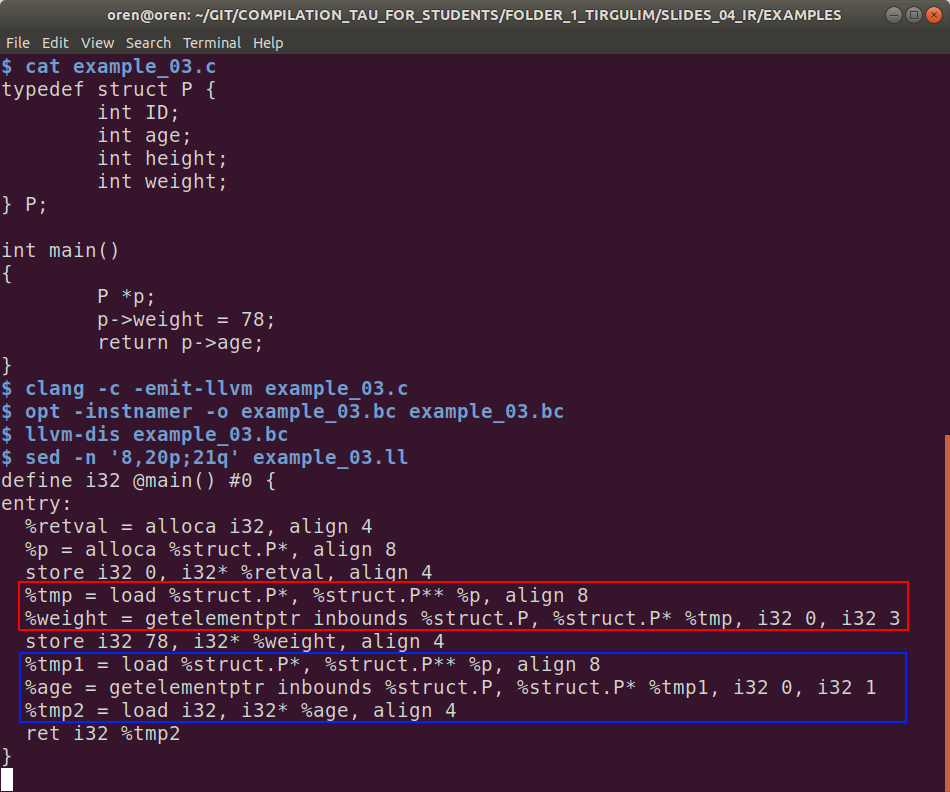
\includegraphics[width=0.95\textwidth]{example_03.png}
\end{center}
\end{column}
\begin{column}{0.6\textwidth}
\begin{itemize}
\item
how to handle p$\rightarrow$weight? ({\color{red} red})
\item
similar to p$\rightarrow$age? ({\color{blue} blue})
\item
handling (field) vars in a\\
uniform way clearly has its
advantages.
\item
However, return p$\rightarrow$age;\\
needs the \textit{value}, and     \\
p$\rightarrow$weight := 78;       \\
needs the \textit{address}
\item
any way to reconcile this?
\end{itemize}
\end{column}
\end{columns}
}